\part{Fonctions et continuité}
\begin{exercice}[Limite à droite, limite à gauche]\label{ex:limits}
Commençons par répondre à la question de la continuité~: remarquons que seules les fonction $h$ et $k$ sont définies au point d'étude. Ainsi, les fonctions $f$, $g$, $i$ et $j$ ne sont pas continues par définition~; il nous reste uniquement à déterminer si $h$ et $k$ sont continues.
\begin{enumerate}
    \item Pour $f(x) = \frac{\tan(x)}{x}$, il nous suffit de remarquer par la définition de la tangente que
    \[
    f(x) = \frac{\tan(x)}{x} = \frac{\sin(x)}{x} \frac{1}{\cos(x)}
    \]
    Or, on a vu lors du cours que $\displaystyle\lim_{x \to 0} \frac{\sin(x)}{x} = 1$, et $\displaystyle\lim_{x \to 0} \cos(x) = \cos(0) = 1$ par la continuité du cosinus, donc par les propriétés des limites~:
    \[
    \lim_{x \to 0} f(x) = \lim_{x \to 0} \underbrace{\frac{\sin(x)}{x}}_{\to 1} \underbrace{\frac{1}{\cos(x)}}_{\to 1} = 1
    \]
    Nul besoin pour cet exemple de différencier la limite à droite et la limite à gauche, car toutes les limites existent des deux côtés.
    
    \item Il nous faut être prudent à cause du terme en $\frac{1}{x-2}$. Par le changement de variable $y = x-2$,
    \[
    \frac{x-1}{x-2} = \frac{y+1}{y} = 1 + \frac{1}{y}
    \]
    Ainsi
    \[
    \lim_{x \to 2^-} \frac{x-1}{x-2} = \lim_{y \to 0^-} 1 + \frac{1}{y} = -\infty \quad \textrm{et} \quad \lim_{x \to 2^+} \frac{x-1}{x-2} = \lim_{y \to 0^+} 1 + \frac{1}{y} = +\infty
    \]
    Les deux limites ne sont pas égales, donc $\displaystyle\lim_{x \to 2} g(x)$ n'est pas définie.
    
    \item Ici, pas de piège ! La fonction $h(x) = \frac{x^3}{3} + 3x^2$ est bien continue en $x = 0$, par combinaison de fonctions continues. Ainsi,
    \[
    \lim_{x \to 0} \frac{x^3}{3} + 3x^2 = h(0) = 0
    \]
    
    \item Notons premièrement qu'il est difficile pour cette fonction d'obtenir de l'intuition autour de $0$. En particulier, plusieurs phénomènes sont en conflits (comment $\sin$ réagit avec $\frac{1}{x}$, comment la multiplication du sinus par $x$ agit-elle, etc.) et donc il est primordial d'avoir une idée de la direction dans laquelle aller.
    
    Le réflexe à avoir avec un sinus est de l'encadrer, pour pouvoir potentiellement appliquer le théorème des gendarmes. De $-1 \leq \sin\left(\frac{1}{x}\right) \leq 1$ on obtient autour de $0$ l'inégalité
    \[
    -x \leq x \sin\left(\frac{1}{x}\right) \leq x
    \]
    Les deux fonctions à gauche et à droite de l'inégalité convergent clairement vers $0$ lorsque $x \to 0$, et ainsi par le théorème des gendarmes~:
    \[
    \lim_{x \to 0} x \sin\left(\frac{1}{x}\right) = 0
    \]
    Ce résultat devient plus clair lorsqu'on affiche le graphique de la fonction, ainsi que les droites d'équations $y = x$ et $y = -x$ (en rouge ci-dessous)~:
    \begin{figure}[H]
    \centering
    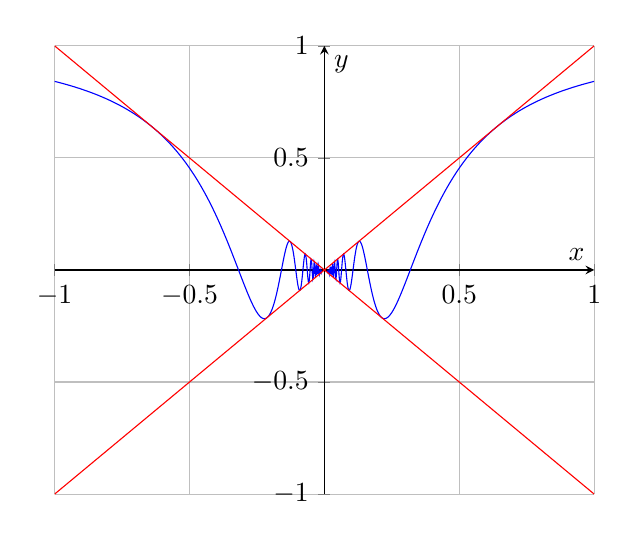
\begin{tikzpicture}
        \begin{axis}[
            xmin = -1,
            ymin = -1,
            xmax = 1,
            ymax = 1,
            xlabel = $x$,
            ylabel = $y$,
            axis lines = middle,
            grid,
            trig format plots=rad
        ]
        
        \addplot[blue, domain=-1:-0.01,samples=600] {x * sin(1/x)};
        \addplot[blue, domain=0.01:1,samples=600] {x * sin(1/x)};
        \addplot[red, domain=-1:1] {x};
        \addplot[red, domain=-1:1]{-x};
        
        \end{axis}
    \end{tikzpicture}
    \caption{Graphe de $i(x) = x \sin\left(\frac{1}{x}\right)$ autour de $0$}
    \label{fig:i_graph}
\end{figure}
    
    
    \item En suivant l'indice donné, on obtient que
    \[
    \lim_{x \to 3} \frac{e^{x-3}-1}{x-3} = \lim_{h \to 0} \frac{e^h - 1}{h}
    \]
    On reconnaît alors -- d'une manière un peu détournée -- la définition de la \emph{dérivée} de $\exp(x) = e^x$ en $x = 0$, puisque $\exp(0) = 1$. Or $\exp'(x) = \exp(x) = e^x$ donc
    \[
    \lim_{x \to 3} \frac{e^{x-3} - 1}{x-3} = \exp'(0) = e^0 = 1
    \]
    
    \item Observons premièrement que la fonction $k$ est \emph{paire}, c'est-à-dire que le graphe de $k$ est symétrique par rapport à la droite verticale $x = 0$, car $k(-x) = k(x)$. Ainsi, $k$ admet le même comportement de part et d'autre de $0$, et donc les limites à droites et à gauche coïncideront vers une unique limite.
    
    Un détail important dans le calcul de la limite en un point est que ce calcul \emph{ne prend jamais en compte la valeur en ce point}, c'est-à-dire qu'on étudie une limite \emph{épointé}, tout autour de $0$ mais pas en $0$. En effet, on a pu calculer des limites autour d'un point où la fonction n'était même pas définie, ce qui prouve que le point $x = 0$ n'influe pas sur la limite. Peu importe donc la valeur de $k(0)$.
    
    On peut calculer désormais notre limite en utilisant ces deux remarques~:
    \[
    \lim_{x \to 0} k(x) = \lim_{x \to 0^+} \sqrt{|x|} = \lim_{x \to 0^+} \sqrt{x} = 0
    \]
    On peut vérifier de même que $\displaystyle\lim_{x \to 0^-} k(x)$ sera aussi 0. Puisque $k$ est définie en 0, on a $\displaystyle\lim_{x \to 0} k(x) \neq k(0) = 1$, donc $k$ n'est pas continue en $0$.
\end{enumerate}
\end{exercice}

\begin{exercice}[Continuité]\label{ex:weird_function}
Cet exercice a pour but de vous faire manipuler les propriétés du logarithme, en particulier ses limites autour de points bien choisis. Rappelons que
\begin{align*}
\lim_{x \to 0^+} \ln(x) & = -\infty \\
\lim_{x \to 1^-} \ln(x) & = 0^- \\
\lim_{x \to 1^+} \ln(x) & = 0^+
\end{align*}
où l'on note $0^-$ et $0^+$ le côté par lequel $0$ est approché. De plus, $\ln(x)$ n'est pas défini pour $x \leq 0$.

La fonction $u$ est continue pour $x \not\in \{-1, 0, 1\}$, par combinaison de fonctions continues. Il nous reste à calculer les limites aux points problématiques~:
\begin{enumerate}
    \item Autour de $x = 0$, on a
    \[
    \lim_{x \to 0^-} \frac{1}{\ln(|x|)} = \lim_{x \to 0^-} \frac{1}{\ln(\underbrace{-x}_{> 0})} = 0
    \]
    De manière similaire, on obtient
    \[
    \lim_{x \to 0^+} \frac{1}{\ln(|x|)} = \lim_{x \to 0^+} \frac{1}{\ln(x)} = 0
    \]
    Notez qu'on aurait pu utiliser le même argument de parité de la fonction $k$ de l'Exercice \ref{ex:limits}, grâce à la valeur absolue.
    On obtient finalement que
    \[
    \lim_{x \to 0} \frac{1}{\ln(|x|)} = 0 = u(0)
    \]
    Donc $u$ est continue en $0$.
    
    \item Autour de $x = \pm 1$, le comportement sera symétrique, i.e.
    \begin{align*}
    \lim_{x \to -1^-} \frac{1}{\ln(|x|)} & = \lim_{x \to -1^-} \frac{1}{\ln(\underbrace{-x}_{\to 1^+})} = +\infty \\
    \lim_{x \to -1^+} \frac{1}{\ln(|x|)} & = \lim_{x \to -1^+} \frac{1}{\ln(\underbrace{-x}_{\to 1^-})} = -\infty \\
    \end{align*}
    par les propriétés mentionnées en rappel. De la même manière,
    \begin{align*}
    \lim_{x \to 1^+} \frac{1}{\ln(|x|)} = \lim_{x \to 1^+} \frac{1}{\ln(x)} = +\infty \\
    \lim_{x \to 1^-} \frac{1}{\ln(|x|)} = \lim_{x \to 1^-} \frac{1}{\ln(x)} = -\infty
    \end{align*}
    Par la divergence des limites, $u$ n'est pas continue en $\pm 1$.
\end{enumerate}
On conclut alors que $u$ est continue pour tout $x \not\in \{-1, 1\}$. Sur le graphe de $u$ ci-dessous, cela correspond exactement aux points où la fonction a un saut. Notez aussi que les limites qu'on a calculé se retrouvent bien visuellement, autour des points $x = -1, 0$ et $-1$~:
\begin{figure}[H]
    \centering
    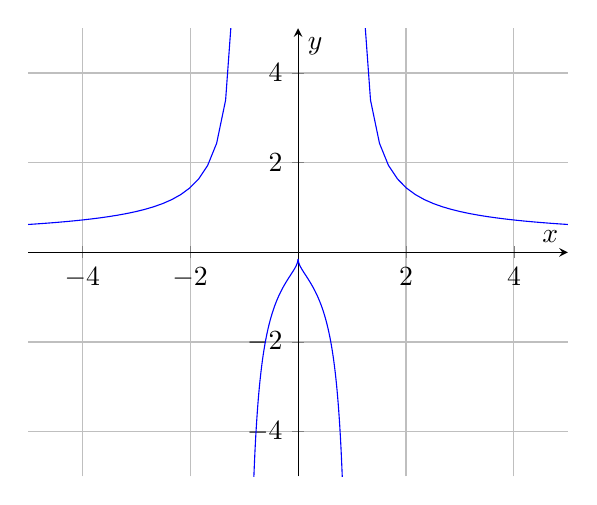
\begin{tikzpicture}
        \begin{axis}[
            xmin = -5,
            ymin = -5,
            xmax = 5,
            ymax = 5,
            xlabel = $x$,
            ylabel = $y$,
            axis lines = middle,
            grid
        ]
        
        \addplot[blue, domain=-5:-1.01] {1 / ln(-x)};
        \addplot[blue, domain=-0.99:0.99, samples = 500] {1 / ln(abs(x))};
        \addplot[blue, domain=1.01:5] {1 / ln(x)};
        
        % \addplot[color=blue,fill=blue,only marks,mark=*] coordinates{(-1,0) (0, 0) (1, 0)};
        
        \end{axis}
    \end{tikzpicture}
    \caption{Graphe de $u$}
    \label{fig:u_graph}
\end{figure}
\end{exercice}

\begin{exercice}[Prolongement par continuité]
Observons premièrement que le prolongement par continuité n'est possible que si~:
\begin{enumerate}
    \item La fonction n'est pas définie au point d'étude, et
    \item La limite existe (i.e. n'est pas infinie/indéfinie).
\end{enumerate}
Ainsi, les fonctions $h$ et $k$ sont déjà définies en $x = 0$, donc il ne fait pas de sens de parler de prolongement. On considère alors les limites obtenus dans l'Exercice~\ref{ex:limits}~:
\begin{enumerate}
    \item Pour $f(x) = \frac{\tan(x)}{x}$, la limite en $0$ est $1$, donc on peut la prolonger par continuité, et son prolongement par continuité est
    \[
    \tilde{f}(x) = \begin{cases}
    \frac{\tan(x)}{x} & \textrm{si } x \neq 0 \\
    1 & \textrm{si } x = 0
    \end{cases}
    \]
    \item $g(x) = \frac{x-1}{x-2}$ n'admet pas de limite réelle en $x = 2$, donc $g$ n'est pas prolongeable par continuité.
    \item $i(x) = x \sin\left(\frac{1}{x}\right)$ a pour limite $0$ en $x = 0$, donc on peut prolonger $i$ par continuité~:
    \[
    \tilde{i}(x) = \begin{cases}
    x \sin\left(\frac{1}{x}\right) & \textrm{si } x \neq 0 \\
    0 & \textrm{si } x = 0
    \end{cases}
    \]
    \item $j(x) = \frac{e^{x-3} - 1}{x-3}$ a pour limite $1$ en $x = 3$, donc son prolongement par continuité est~:
    \[
    \tilde{j}(x) = \begin{cases}
    \frac{e^{x-3} - 1}{x-3} & \textrm{si } x \neq 3 \\
    1 & \textrm{si } x = 3
    \end{cases}
    \]
\end{enumerate}
\end{exercice}

\begin{exercice}[Théorème des valeurs intermédiaires]
\enumeratelinefix
\begin{enumerate}
    \item Observons tout d'abord que la fonction $l$ peut se réécrire comme
    \[
    l(x) = x^3 - 3x^2 + 3x - 1 = (x-1)^3
    \]
    $l$ est évidemment continue sur $[0, 3]$, et c'est aussi une fonction croissante (sa dérivée étant $l'(x) = 3(x-1)^2 \geq 0$ pour $x \in [0, 3]$). Ainsi, son minimum est atteint en $x = 0$, avec $f(0) = -1$, et son maximum est atteint en $x = 3$, avec $f(3) = 2^3 = 8$. Par le Théorème des valeurs intermédiaires, son image est donc~:
    \[
    f([0, 3]) = [-1, 8]
    \]
    
    \item Attention, la fonction $m(x) = \frac{1}{x}$ n'est pas continue en $0$, donc en particulier elle n'est pas continue sur $[-1, 1]$ ! Il nous est impossible d'appliquer directement le Théorème des valeurs intermédiaires (abrégé T.V.I), et il nous faut procéder autrement.
    
    Notons $I = [-1, 0[$. $m$ est bien continue sur $I$ -- elle est même continue pour tout intervalle de la forme $[-1, a]$ avec $-1 < a < 0$. Sur ces intervalles, il est possible d'appliquer le T.V.I pour trouver que l'image est~:
    \[
    m([-1, a]) = \left[\frac{1}{a}, -1\right]
    \]
    Intuitivement, si on fait tendre $a$ vers $0^-$, on voit bien alors que 
    \[
    m([-1, 0[) = m(I) = \,]\!-\!\infty, -1]
    \] puisque $\displaystyle\lim_{a \to 0^-} \frac{1}{a} = -\infty$. Pour le prouver plus formellement, il nous suffit de montrer que~:
    \begin{enumerate}
        \item Pour tout $x \in I$, $m(x) \leq -1$, et
        \item Pour tout $y \leq -1$, il existe $x \in I$ tel que $m(x) = y$.
    \end{enumerate}
    
    Prouvons d'abord que $m(x) \leq -1$ pour tout $x \in I$. Il est aisé de voir que $m$ est une fonction décroissante sur $I$, et ainsi
    \[
    -1 \leq x < 0 \implies m(-1) = -1 \geq m(x)
    \]
    ce qui prouve notre inégalité. Pour prouver la surjectivité, observons que
    \[
    m(x) = \frac{1}{x} = y \iff x = \frac{1}{y}
    \]
    Or $y \leq -1 \implies x = \frac{1}{y} \geq -1$ par décroissance de $m$, donc $x \in I$. On a ainsi trouvé $x \in I$ tel que $m(x) = y$, ce qui prouve bien que l'image de $[-1, 0[$ par $m$ est $]\!-\!\infty, -1]$.
    
    Par un raisonnement similaire, on trouve que l'image de $m$ sur l'intervalle $J = ]0, 1]$ est $[1, \infty[$, et ainsi on obtient que
    \[
    m([-1, 1]) = ]\!-\!\infty, -1] \cup [1, \infty[
    \]
    
    \item Notons premièrement que la fonction $n(x) = \tan(x) = \frac{\sin(x)}{\cos(x)}$ n'est pas définie pour $\cos(x) = 0$, i.e. si $x = k\pi + \frac{\pi}{2}$ pour $k \in \mathbb{Z}$. Puisque l'intervalle $I = [-\frac{\pi}{4}, \frac{\pi}{3}]$ ne contient pas de tels points, $n$ est continue sur tout l'intervalle, par quotient de fonctions continues. Ainsi, il nous suffit de trouver le maximum et le minimum de $n$ sur $I$. On peut remarquer que $\tan$ est une fonction croissante, puisque
    \[
    \tan'(x) = \frac{1}{\cos(x)^2} \geq 0
    \]
    pour tout $x \in I$ (cf. Exercice 7), et ainsi le minimum et le maximum sont respectivement
    \[
    n\left(-\frac{\pi}{4}\right) = \frac{-\frac{\sqrt{2}}{2}}{\frac{\sqrt{2}}{2}} = -1 \quad \textrm{et} \quad n\left(\frac{\pi}{3}\right) = \frac{\frac{\sqrt{3}}{2}}{\frac{1}{2}} = \sqrt{3}
    \]
    Ainsi, par le TVI on conclut que
    \[
    n(I) = [-1, \sqrt{3}]
    \]
\end{enumerate}
\end{exercice}

\begin{exercice}[Fonctions continues et nombre de solutions]
Soit $f(x) = x^3 - 2x - 1 - \sin(x)$, pour $x \in [-\pi, \pi]$. Notons que $f$ est continue (par somme de fonctions continues), et que
\[
x^3 - 2x - 1 = \sin(x) \iff f(x) = 0
\]
Ainsi, il nous suffit d'appliquer de trouver $a, b \in [-\pi, \pi]$ tels que $f(a) \leq 0$ et $f(b) \geq 0$ pour pouvoir appliquer le théorème des valeurs intermédiaires et conclure sur l'existence d'au moins une solution.

\smallskip
\noindent Par tâtonnements, on peut trouver les paires suivantes :
\begin{enumerate}
    \item $f(-\pi) = -\pi^3 - 2\pi - 1 < 0$ et $f(-1) = - \sin(-1) = \sin(1) > 0$, donc il existe (au moins) une solution $x_1 \in ]-\pi, -1[$.
    \item $f(0) = - 1 - \sin(0) = -1 < 0$, donc il existe (au moins) une solution $x_2 \in ]-1, 0[$.
    \item $f(\pi) = \pi^3 - 2\pi - 1 > 3^3 - 2\cdot 3 - 1 > 0$, donc il existe (au moins) une solution $x_3 \in ]0, \pi[$.
\end{enumerate}
Ainsi, on a bien au minimum 3 solutions, comme on peut le voir sur le graphique de $f$~:
\begin{figure}[H]
    \centering
    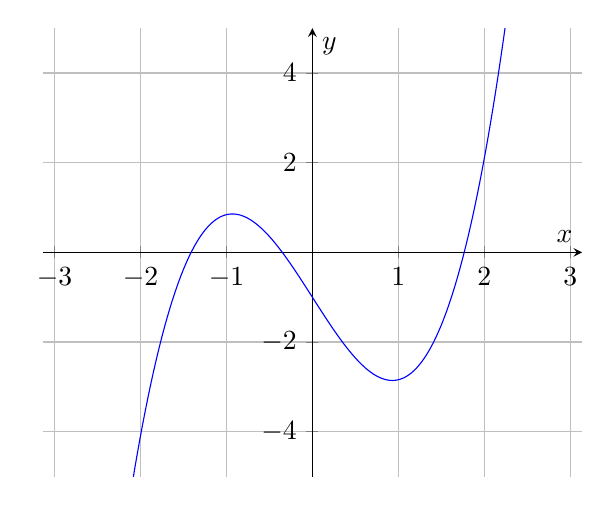
\begin{tikzpicture}
        \begin{axis}[
            xmin = -3.14,
            xmax = 3.14,
            ymin = -5,
            ymax = 5,
            xlabel = $x$,
            ylabel = $y$,
            axis lines = middle,
            grid,
            trig format plots=rad
        ]
        
        \addplot[blue, domain=-3.14:3.14,samples=200] {x * x * x - 2 * x - 1 - sin(x)};
        
        \end{axis}
    \end{tikzpicture}
    \caption{Graphe de $f(x) = x^3 - 2x - 1 - \sin(x)$ sur $[-\pi, \pi]$}
    \label{fig:solutions_graph}
\end{figure}
\end{exercice}